\documentclass{beamer}

%\usetheme{Boadilla}

\usepackage{graphics}
\usepackage{amsmath}
\usepackage{listings}

%--------------------------------------------------
% Macros

\newcommand{\vf}[1]{\vskip0pt plus #1}

%--------------------------------------------------
% Beamer stuff
\usefonttheme{structurebold}
\useinnertheme{default}
\useoutertheme{smoothbars}

% hacked albatross color theme
\setbeamercolor*{normal text}{fg=yellow!20!white,bg=blue!0!black}

\setbeamercolor*{example text}{fg=green!65!black}

\setbeamercolor*{structure}{fg=blue!25!white}

\setbeamercolor{palette primary}{use={structure,normal text},fg=structure.fg,bg=normal text.bg!75!black}
\setbeamercolor{palette secondary}{use={structure,normal text},fg=structure.fg,bg=normal text.bg!60!black}
\setbeamercolor{palette tertiary}{use={structure,normal text},fg=structure.fg,bg=normal text.bg!45!black}
\setbeamercolor{palette quaternary}{use={structure,normal text},fg=structure.fg,bg=normal text.bg!30!black}

\setbeamercolor*{block body}{bg=normal text.bg!90!black}
\setbeamercolor*{block body alerted}{bg=normal text.bg!90!black}
\setbeamercolor*{block body example}{bg=normal text.bg!90!black}
\setbeamercolor*{block title}{parent=structure,bg=normal text.bg!75!black}
\setbeamercolor*{block title alerted}{use={normal text,alerted text},fg=alerted text.fg!75!normal text.fg,bg=normal text.bg!75!black}
\setbeamercolor*{block title example}{use={normal text,example text},fg=example text.fg!75!normal text.fg,bg=normal text.bg!75!black}

\setbeamercolor{item projected}{fg=black}

\setbeamercolor*{sidebar}{parent=palette primary}

\setbeamercolor{palette sidebar primary}{use=normal text,fg=normal text.fg}
\setbeamercolor{palette sidebar secondary}{use=structure,fg=structure.fg}
\setbeamercolor{palette sidebar tertiary}{use=normal text,fg=normal text.fg}
\setbeamercolor{palette sidebar quaternary}{use=structure,fg=structure.fg}

\setbeamercolor*{separation line}{}
\setbeamercolor*{fine separation line}{}



%\usecolortheme{orchid} % inner color theme
%\usecolortheme{seahorse} % outer color theme
%\usecolortheme{albatross}
%\usecolortheme[rgb={0.7,0.4,0.1}]{structure}
%\usecolortheme[hsb={0.6,0.4,0.55}]{structure}
%\usecolortheme[hsb={0.6,0.4,0.45}]{structure}
%\setbeamercolor{background canvas}{bg=}

\usefonttheme[onlymath]{serif}
%\usefonttheme[stillsansseriftext,stillsansserifsmall]{serif}

\setbeamercovered{transparent}

\setbeamertemplate{navigation symbols}{}

\title[Interactive fractal flames]{Interactive fractal flames with CUDA and OpenGL}
%\titlegraphic{\includegraphics[viewport=8 653 558 831,width=6cm]{figures/logos.pdf}}
%\subtitle{}


\author{Chris Foster}
\institute{ROAMES}
\date{March 22, 2011}


%===============================================================================
%===============================================================================
\begin{document}

\begin{frame}[plain]
  \titlepage
\end{frame}

%\begin{frame}
%  \frametitle{Overview}
%  \tableofcontents
%\end{frame}


%===============================================================================
\section{Introduction}

\begin{frame}
  \frametitle{What is a fractal?}
  \begin{itemize}
    \item
      Fractional (Hausdorff) dimension $>$ topological dimension. \\
      Power law for number of covering boxes: $N(\epsilon) \sim 1/\epsilon^D$
    \item
      (Quasi-) self-similar at all scales
  \end{itemize}
  \vf{10filll}
\end{frame}



%===============================================================================
\section{Mathematics}

\begin{frame}
  \frametitle{Iterated function systems (IFS)}
  \begin{itemize}
    \item
      Hutchinson 1981 \cite{Hutchinson1981}: general set of strictly 
      self-similar fractals
    \item
      Popularised by Barnsley \cite{Barnsley1988} in \emph{Fractals Everywhere}, 1988
    \item
      Set of $N$ contractive functions $F_i \colon \mathbb{R}^2\to\mathbb{R}^2$
    \item
      ``Attractor'' obeys recursive set equation
      \[
      A_{k+1} = \bigcup_{i=1}^N F_i(A_k) \qquad
      A_k \to A \;\;\text{as}\;\; k \to \infty
      \]
    \item
      $F_i$ traditionally \emph{affine} (rotation/translation/scaling)
  \end{itemize}
  \vf{1filll}
\end{frame}


\begin{frame}
  \frametitle{Flame Fractals}
  \onslide+<1>
  \begin{itemize}
    \item
      Invented by Draves \& Reckase 2003 \cite{Draves2003} (flam3/electric sheep)
    \item
      Non-affine $F_i$: more artistic flexibility
      \[
      F_i = P_i\bigg(\sum_m v_{im} V_m\big(Q_i(x,y)\big)\bigg)
      \]
    \item
      $V_m$ are nonlinear ``variations''; maps $P_i$ and $Q_i$ are affine:
      \[
        Q_i(x,y) = \big(a_i x + b_i y + c_i,\; d_i x + e_i y + f_i \big)
      \]
  \end{itemize}
  \vf{10fill}
  \onslide<2>
\end{frame}


%===============================================================================
\section{Implementation}

\begin{frame}[fragile]
  \frametitle{Monte Carlo sampling}
  \lstset{language=python,basicstyle=\scriptsize}
\begin{lstlisting}
P = (0,0,0)    # Arbitrary position
C = (0,0,0)    # Arbitrary colour

for i in range(0,maxIter):
    func = choose_function_at_random(funcs)
    P = func(P)
    C = 0.5*(func.C + C)
    if i > discardCutoff:
        plot_point(P, C)
\end{lstlisting}
  \vf{5filll}
\end{frame}


\begin{frame}
  \frametitle{Implementation overview}
  \begin{itemize}
    \item
      Generate point list using CUDA
    \item
      Render points with additive OpenGL blending
    \item
      HDR tone mapping and gamma correction
  \end{itemize}
  \vf{5filll}
\end{frame}


\begin{frame}
  \frametitle{GPU flames}
  \begin{itemize}
    \item
      History: S. Green \cite{Green2005}, flam4 (keldor314), GPU gems \cite{Schied2011}
    \item
      My implementation in CUDA is pretty naive:
    \item
      50 points from each of 40,000 threads (total 2,000,000) generated into 
      vertex buffer object
    \item
      curand for random numbers
  \end{itemize}
  \vf{1filll}
\end{frame}


\begin{frame}
  \frametitle{OpenGL High Dynamic Range Pipeline}
  \begin{itemize}
    \item
      Accumulate into offscreen float-precision FBO
    \item
      Tone mapping \& gamma correction with GLSL:
      \[
      \text{RGB}_{\text{linear}}\to \text{xyY} \to \text{xyY}' \to
      \text{RGB}'_{\text{linear}} \to \text{RGB}'_{\text{gamma}}
      \]
  \end{itemize}
  \onslide+<1>
  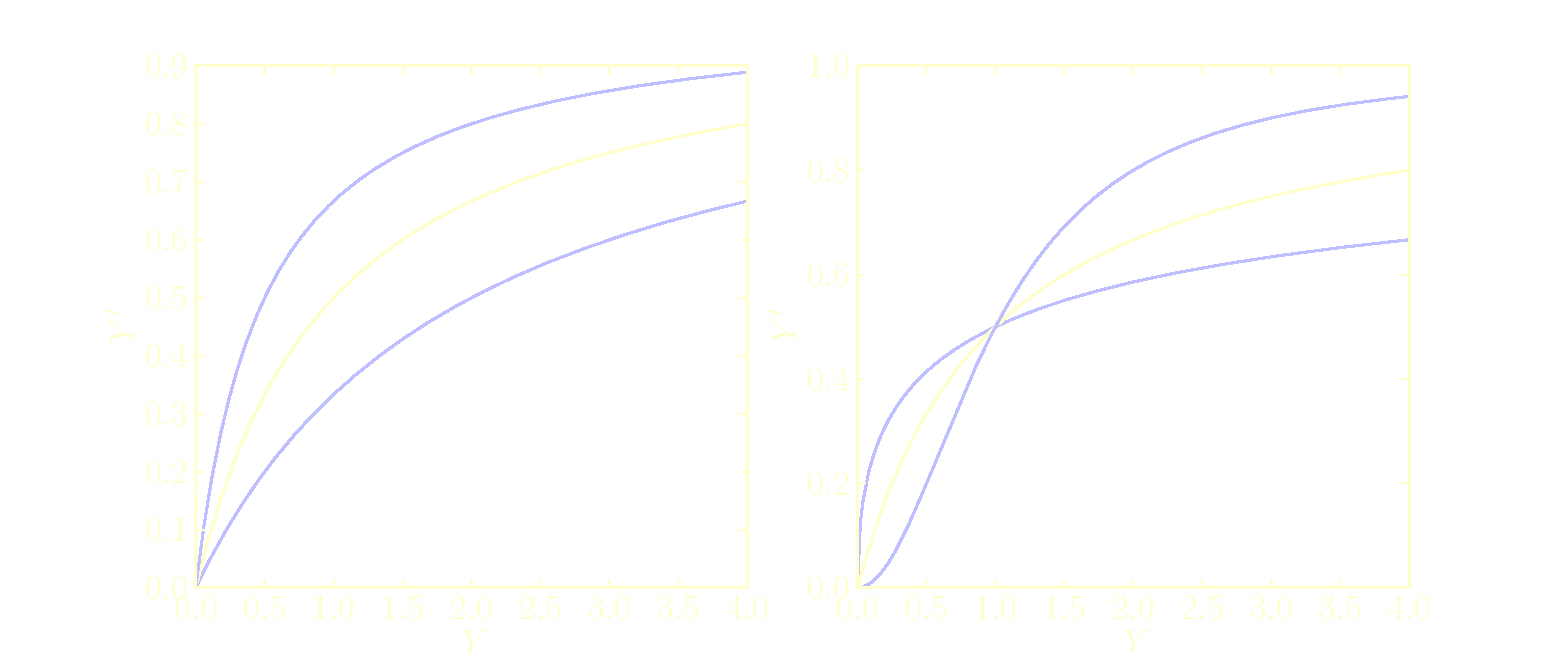
\includegraphics[width=10cm]{tone_map.pdf}
  \onslide<2>
\end{frame}


\begin{frame}[fragile]
  \frametitle{Future Performance Tuning}
  \begin{itemize}
    \item
      Warp divergence with many variations and many functions
    \item
      GPU gems algorithm \cite{Schied2011}
  \end{itemize}
  \vf{5filll}
\end{frame}



%===============================================================================
\section*{End}

\begin{frame}[fragile]
  %Thanks (collage)

  \vf{1filll}
  \verb|www.github.com/c42f/flamed|
  \vskip1em
\end{frame}


\begin{frame}
  \frametitle{References}
  \nocite{*}
  \bibliographystyle{unsrt}
  \fontsize{7pt}{7pt}
  \bibliography{bibliography}
  \normalsize
\end{frame}



%===============================================================================
%===============================================================================
%\part{Extras}
%
%\begin{frame}
%  \frametitle{GLSL HDRI}
%  \lstset{language=C,basicstyle=\tiny}
%  \lstinputlisting[linerange=2-16]{../hdri.glsl}
%\end{frame}


%\begin{frame}
%  \frametitle{Collage Theorem}
%\end{frame}


\end{document}
